\chapter{ModeloDinamico}	


	Este capítulo describe en modelo dinámico del sistema. en el se detallan todos los escenarios de ejecución del sistema. La figura~\ref{fig:casosDeUso} muestra el diagrama general del sistema y todos sus casos de uso.

%---------------------------------------------------------
\section{Descripción de actores}

%---------------------------------------------------------DUEÑO
\begin{Usuario}{\hypertarget{Dueño}{\subsection{Dueño}}}{
	Es el encargado de todas las operaciones de mayor importancia de las farmacias
	se encarga de contratar al personal, tanto empleados como supervisores y también controla las sucursales de la farmacia.
}
    \item[Responsabilidades:] \cdtEmpty
    \begin{itemize}
		\item Contratar Personal y asignarlo a una sucursal.
		\item Asignar  sucursales.
		\item Crear paquetes de descuento.
		\item Dar de baja Personal.
		\item Cerrar sucursales.
		\item Agregar nuevos tipos de medicamentos al sistema.
		\item Dar de baja paquetes de descuento.
		\item Modificar los medicamentos en los paquetes de descuento.
		\item Controlar los permisos en el sistema.
		\item Conocer al personal.	
    \end{itemize}
\end{Usuario}

%---------------------------------------------------------Supervisor
\begin{Usuario}{\hypertarget{Supervisor}{\subsection{Supervisor}}}{
	Es el encargado de llevar un control de la apertura y cierre de turno,
	así como hacer un reporte de ventas mensuales al dueño sobre las sucursales en las que esta asignado.
}
    \item[Responsabilidades:] \cdtEmpty
    \begin{itemize}
		\item Dar de baja medicamentos estropeados.
		\item Supervisar a los empleados.
		\item Abrir turno del cajero.
		\item Cerrar turno del cajero.
		\item Cambiar los datos de los medicamentos que estén registrados de forma incorrecta.
    \end{itemize}
    
	\item[Perfil:] \cdtEmpty
    \begin{itemize}
		\item Amplia experiencia en el rama de farmacias.
		\item Licenciatura como mínimo.
    \end{itemize}
\end{Usuario}

%---------------------------------------------------------Empleado
\begin{Usuario}{\hypertarget{Empleado}{\subsection{Cajero}}}{
	Es el encargado de realizar la ventas, atender proveedores y clientes
}
    \item[Responsabilidades:] \cdtEmpty
    \begin{itemize}
		\item Registra medicamentos del proveedor.
		\item Realiza ventas.
		\item Aplica descuentos de los paquetes hechos por el dueño.
		\item Registrar datos de clientes en el sistema.
		\item Hacer devoluciones.
		\item Dar créditos al cliente con los cuales se puede comprar medicina.
		\item Conocer los medicamentos que se tienen en su sucursal a si como la cantidad de cada medicamento.
    \end{itemize}

	\item[Perfil:] \cdtEmpty
    \begin{itemize}
		\item Bachillerato terminado.
		\item Responsable
		\item Honesto
    \end{itemize}
\end{Usuario}
A continuación se detallan los casos de uso.

%---------------------------------------------------------
\begin{figure}[htbp]
	\begin{center}
		\fbox{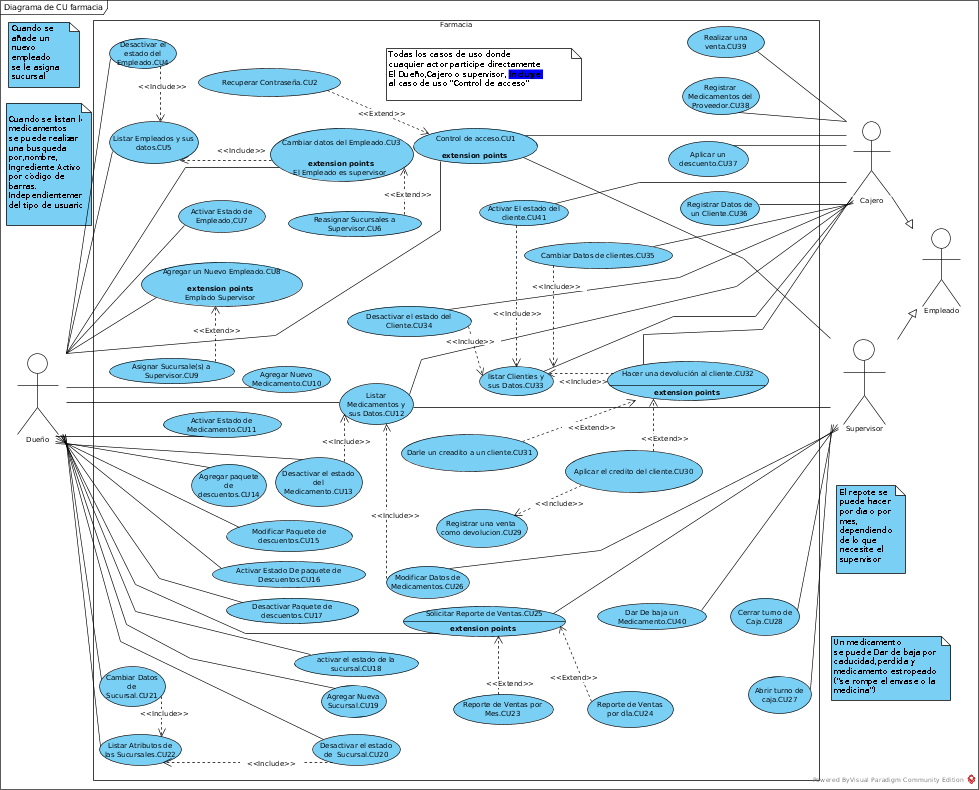
\includegraphics[width=18cm, height=20cm]{images/DiagramaCU}}
		\caption{Diagrama de casos de uso del sistema.}
		\label{fig:casosDeUso}
	\end{center}
\end{figure}

%CASOS DE USO
Esencia de los Casos de Uso.
 \begin{UseCase}{CU1}{Control de Acceso}{
		Operacion inicia para poder acceder al sistema. De éste Caso de uso se extiende a todos los demás casos de uso.
	}
		\UCitem{Versión}{\color{Gray}0.1}
		\UCitem{Autor}{\color{Gray}Aguilera Rosas Landa Enrique}
		\UCitem{Supervisa}{\color{Gray}.}
		\UCitem{Actor}{Cajero,Supervisor,Dueño}
		\UCitem{Propósito}{Ingresar al Sistema para poder Realizar Transacciones diarias de la farmacia}
		\UCitem{Entradas}{Direccion URL de la pagina web de la farmacia,Contraseña y Correo Electrónico}
		\UCitem{Origen}{Teclado}
		\UCitem{Salidas}{Pantalla principal Dependiendo del tipo de Usuario \IUref{IU1}{Pantalla Principal Dueño}\IUref{IU2}{Pantalla Principal Supervisor}\IUref{IU3}{Pantalla Principal Cajero}}
		\UCitem{Destino}{Pantalla}
		\UCitem{Precondiciones}{Se debe introducir la direccion de la pagina en el navegador de internet }
		\UCitem{Postcondiciones}{El Empleado,Supervisor o Dueño podrá hacer transacciones de su índole}
		\UCitem{Errores}{Que la pagina no este disponible por razones tales de: Error de conexion, Mantenimiento de los servidores, Que no exista el usuario,Que la contraseña este Incorrecta,Que no exista el correo electrónico}
		\UCitem{Observaciones}{}
		\UCitem{Estado}{En revision}
	\end{UseCase}
%--------------------------------------
	\begin{UCtrayectoria}{Principal}
		\UCpaso[\UCactor] Ingresa a la pagina web escribiendo la URL en un navegador.
		\UCpaso Genera Y despliega la Pantalla \IUref{IU0}{Login}
		\UCpaso [\UCactor] Ingresa su Correo Electronico y Contraseña y presiona el boton Aceptar
		\UCpaso Verifica que el [\UCactor] haya haya proporcionado los datos requeridos en la pantalla \IUref{IU0}{Login}
		\UCpaso Verifica que el correo proporcionado cumpla con el formato XXXX@XXX.XXX \Trayref{A}
		\UCpaso Busca la cuenta asociada al correo ingresado. \Trayref{B}
		\UCpaso Verifica que dicha cuenta este activa. \Trayref{C}
		\UCpaso Verifica que la contraseña ingresada coincida con la contraseña asociada a la cuenta.\Trayref{F}
		\UCpaso Otorga el acceso al sistema
		\UCpaso Muestra la pantalla correspondiente al tipo de cuenta.		
		\UCpaso [\UCactor] Usa el sistema.
		\UCpaso [\UCactor] Solicita cerrar sesión.
		\UCpaso Revoca el acceso.
		\UCpaso Muestra \IUref{IU1}{Login}		
	\end{UCtrayectoria}

%--------------------------------------		
	\begin{UCtrayectoriaA}{A}{El Correo no esta Correcto}
			\UCpaso Muestra el Mensaje {\bf MSG03-}`` [{\em correo con formato incorrecto}] Introduzca un correo con el formato xxx@xx.xx .''.
			\UCpaso Continúa en el paso 3 del \UCref{CU1}.
		\end{UCtrayectoriaA}
%----------------------------------------
		\begin{UCtrayectoriaA}{B}{El \UCactor no esta registrado}
			\UCpaso Muestra el Mensaje {\bf MSG01-}``Error [{\em Usuario no Encontrado}] El usuario y/o contraseña no existen .''.
			\UCpaso[\UCactor] Oprime el botón \IUbutton{Aceptar}.
			\UCpaso[] Continua en el paso 3 del \UCref{CU1}.
		\end{UCtrayectoriaA}		
%--------------------------------------
		\begin{UCtrayectoriaA}{C}{La cuenta a la que intenta acceder no esta activa}
			\UCpaso Muestra el Mensaje {\bf MSG02-}``Error [{\em Cuenta Desactivada}] Contacta con el Dueño para resolver el problema .''.
			\UCpaso[\UCactor] Oprime el botón \IUbutton{Aceptar}
			\UCpaso Continua en el paso 3 del \UCref{CU1}.
		\end{UCtrayectoriaA}
%--------------------------------------
		\begin{UCtrayectoriaA}{F}{La Contraseña es incorrecta}
			\UCpaso Muestra el Mensaje {\bf MSG06-}`` [{\em Contraseña invalida}] La contraseña ingresada no coincide con la cuenta.''.
			\UCpaso Continúa en el paso 2 del \UCref{CU1}.
		\end{UCtrayectoriaA}
 % control de acceso
\begin{UseCase}{CU2}{Recuperar Contraseña}{
		El empleado puede cometer la equivocación de perder la contraseña asociada a la cuenta con la que ingresa al sistema, por lo cual se requiere de una forma para poder recuperar la contraseña. La recuperación de realizara mediante un correo electrónico el cual se le enviara al empleado con la posibilidad de reasignar una nueva contraseña
	}
		\UCitem{Versión}{\color{Gray}0.1}
		\UCitem{Autor}{\color{Gray}Enrique Aguilera Rosas Landa}
		\UCitem{Supervisa}{\color{Gray}}
		\UCitem{Actor}{\hyperlink{Empleado}{Dueño}}
		\UCitem{Propósito}{Conceder el acceso al sistema de nuevo mediante la recuperación de la contraseña.}
		\UCitem{Entradas}{Correo Electrónico.}
		\UCitem{Origen}{Teclado}
		\UCitem{Salidas}{Contraseña Asociada con la cuenta.}
		\UCitem{Destino}{Pantalla}
		\UCitem{Precondiciones}{El empleado debe estar registrado en el sistema y que no recuerde su contraseña asociada .}
		\UCitem{Postcondiciones}{El empleado recuperara su contraseña y su acceso al sistema.}
		\UCitem{Errores}{Que el acceso a la pagina sea incorrecto debido a razones de Errores De conexión o Mantenimiento de los Servidores, Que el usuario no este registrado en el sistema}

		\UCitem{Observaciones}{¿Que es el formato xxxx@xxx.xx?, Las referencias a las patallas no son, paso 9: link a donde me lleva?,solo existe una pantalla principal, y se llama pantalla principal, pero dependiendo de los permisos que se tengan una opciones del escritorio estaran desabilitadas.los mensajes de bitacora estan en slack para que referencies esos.
		lo démas lo veo bien.}
		\UCitem{Estado}{Corrección}
	\end{UseCase}
%--------------------------------------
	\begin{UCtrayectoria}{Principal}
		\UCpaso Se extiende del caso de uso \UCref{CU0} paso 10.
		\UCpaso[\UCactor] Selecciona la Opción de Recuperación de contraseña dando click en el botón \IUbutton{Recuperar Contraseña}.

		\UCpaso Genera y despliega la pantalla \IUref(04){Recuperación de Contraseña}
		\UCpaso [\UCactor] Proporciona su Correo Electrónico asociado a la contraseña perdida y  Confirma la operación presionando el botón 			\IUbutton{Aceptar}.		
		\UCpaso Verifica que el correo proporcionado cumpla con el formato XXXX@XXX.XXX \Trayref{A}
		\UCpaso Busca la cuenta asociada al correo ingresado. \Trayref{B}
		\UCpaso Verifica que dicha cuenta este activa. \Trayref{C}.
		\UCpaso Envía un correo electrónico al correo proporcionado; el cual contara con un link para asignar una nueva contraseña. \Trayref{D}.
		\UCpaso Redirecciona al \UCactor a la  \IUref{IU1}{Pantalla Principal Dueño}.
	\end{UCtrayectoria}

%--------------------------------------		
	\begin{UCtrayectoriaA}{A}{El Correo no esta Correcto}
			\UCpaso Muestra el Mensaje {\bf MSG03-}`` [{\em correo con formato incorrecto}] Introduzca un correo con el formato xxx@xx.xx .''.
			\UCpaso Continúa en el paso 3 del \UCref{CU2}.
		\end{UCtrayectoriaA}
%----------------------------------------
		\begin{UCtrayectoriaA}{B}{El \UCactor no esta registrado}
			\UCpaso Muestra el Mensaje {\bf MSG01-}``Error [{\em Usuario no Encontrado}] El usuario y/o contraseña no existen .''.
			\UCpaso[\UCactor] Oprime el botón \IUbutton{Aceptar}.
			\UCpaso[] Continua en el paso 3 del \UCref{CU2}.
		\end{UCtrayectoriaA}		
%--------------------------------------
		\begin{UCtrayectoriaA}{C}{La cuenta a la que intenta acceder no esta activa}
			\UCpaso Muestra el Mensaje {\bf MSG02-}``Error [{\em Cuenta Desactivada}] Contacta con el Dueño para resolver el problema .''.
			\UCpaso[\UCactor] Oprime el botón \IUbutton{Aceptar}
			\UCpaso Continua en el paso 3 del \UCref{CU2}.
		\end{UCtrayectoriaA}
%--------------------------------------
	\begin{UCtrayectoriaA}{D}{Correo Electrónico de recuperación de contraseña no se envió}
			\UCpaso Muestra el Mensaje {\bf MSG04-}``Error [{\em Correo no enviado}] Revisa tu conexión y vuelve a enviar el mensaje .''.
			\UCpaso[\UCactor] Oprime el botón \IUbutton{Aceptar}
			\UCpaso Continua en el paso 7 del \UCref{CU2}.
		\end{UCtrayectoriaA}
%--------------------------------------


		
 % Recuperar Contaseña
\begin{UseCase}{CU3}{Modificar datos de  Empleado}{
		Los datos del empleado se tienen que modificar, por inconsistencia en los datos registrados en el sistema con sus datos actuales
	}
		\UCitem{Versión}{\color{Gray}0.1.2}
		\UCitem{Autor}{\color{Gray}Aguilera Rosas Landa Enrique}
		\UCitem{Supervisa}{\color{Gray}Correa Medina Carlos Miguel}
		\UCitem{Actor}{\hyperlink{Alumno}{Dueño}}
		\UCitem{Propósito}{Evitar problemas con los empleados por datos erróneos guardados en el sistema.}
		\UCitem{Entradas}{Nombre completo del solicitante, Edad, Dirección, Curp, RFC, Experiencia Laboral, Puesto , Sucursal}
		\UCitem{Origen}{Teclado}
		\UCitem{Salidas}{No Aplica.}
		\UCitem{Destino}{Pantalla}
		\UCitem{Precondiciones}{El empleado debe de estar dado de alta en el sistema.}
		\UCitem{Postcondiciones}{Los datos del empleado serán diferentes.}
		\UCitem{Errores}{Exista algún duplicado en los datos del empleado, sus cambios no sean guardados}
		\UCitem{Observaciones}{En las Entradas: La experiencia laboral no es un atributo de los empleados, no se como se toma en cuenta ese parametro en el sistema.,paso 1: no exitende del CU0 lo incluye.paso 6: no hay botón que diga modificar empleado en las opciones,paso 7,8:no genera una tabla, muestra el formulario pero con los campos llenos ese formulario se encuentra en slack seccion de #modulo-de-interacción, el boton es {Actualizar} en lugar de {aceptar y guardar} solo existe una pantalla principal, no hay de dueño,empleado o supervisor, solo se controlan las opciones que se pueden hacer pero la pantalla es la misma.}
		\UCitem{Estado}{Corrección}
	\end{UseCase}
%--------------------------------------
	\begin{UCtrayectoria}{Principal}
		\UCpaso Se extiende del caso de uso \UCref{CU0} paso 11
		\UCpaso[\UCactor] Selecciona La opción de ver Lista de  Empleados presionando el botón \IUbutton{Ver Lista de Empleado}.
		\UCpaso Incluye el caso de uso \UCref{CU5}.
		\UCpaso[\UCactor] Introduce el Nombre del empleado a buscar en el campo de Búsqueda \Trayref{A} .
		\UCpaso Genera y Despliega una lista que coincida con la búsqueda realizada
		\UCpaso[\UCactor] Selecciona la opción modificar datos Del empleado Deseado presionando\IUbutton{Modificar Datos}.
		\UCpaso Genera y despliega una tabla con los datos actuales del empleado.
		\UCpaso Genera el formulario Datos del empleado y los despliega.
		\UCpaso[\UCactor] Cambia los datos que el empleado necesita modificar y guarda los cambios presionando el botón \IUbutton{Aceptar y Guardar} \Trayref{B}.
		\UCpaso Redirige al [\UCactor] a la  \IUref{01}{Pantalla Principal de Dueño}.
	\end{UCtrayectoria}


%-------------------------------------------------------------------------


\begin{UCtrayectoriaA}{A}{Empleado no encontrado.}
			\UCpaso Muestra el Mensaje {\bf MSG8-}`` [{\em Empleado no encontrado}] revisa que los campos sean llenados correctamente.''.
			\UCpaso Continúa en el paso \ref{CU7Bus} del \UCref{CU3}.
		\end{UCtrayectoriaA}
%-------------------------------------------------------------------------


\begin{UCtrayectoriaA}{B}{Algún campo del Empleado tiene un error.}
			\UCpaso Muestra el Mensaje {\bf MSG7-}`` [{\em Error en un dato del Empleado}] revisa que los campos sean llenados correctamente.''.
			\UCpaso Continúa en el paso 9 del \UCref{CU3}.
		\end{UCtrayectoriaA}
 % Cambiar datos de empleado
\begin{UseCase}{CU4}{Desactivar estado de  Empleado}{
		Por razones laborales, es mejor desactivar el estado de un empleado que eliminarlo y revocar el acceso al sistema
	}
		\UCitem{Versión}{\color{Gray}0.1.3}
		\UCitem{Autor}{\color{Gray}Aguilera Rosas Landa Enrique}
		\UCitem{Supervisa}{\color{Gray}Correa Medina Carlos Miguel}
		\UCitem{Actor}{\hyperlink{Alumno}{Dueño}}
		\UCitem{Propósito}{Revocar acceso al sistema del empleado.}
		\UCitem{Entradas}{Nombre del Empleado, Id de Empleado}
		\UCitem{Origen}{Teclado}
		\UCitem{Salidas}{No Aplica.}
		\UCitem{Destino}{Pantalla}
		\UCitem{Precondiciones}{El empleado debe de estar registrado en el sistema y con un estado activo.}
		\UCitem{Postcondiciones}{El empleado perderá su acceso al sistema y su estado cambiara a desactivado .}
		\UCitem{Errores}{La pagina sea inaccesible por el momento debido a fallas con los servidores, Que el empleado tenga su cuenta desactivada}
		\UCitem{Observaciones}{}
		\UCitem{Estado}{En Corrección}
	\end{UseCase}
%--------------------------------------
	\begin{UCtrayectoria}{Principal}
		\UCpaso Incluye el caso de uso \UCref{CU1} paso 11
		\UCpaso[\UCactor] Selecciona La opción de ver Lista de  Empleados presionando el botón \IUbutton{Ver Lista de Empleado}.
		\UCpaso[\UCactor] Introduce el Nombre del empleado a buscar en el campo de Búsqueda y presiona el botón \IUbutton{Buscar} \Trayref{A} .
		\UCpaso Genera y Despliega una lista que coincida con la búsqueda realizada
		\UCpaso[\UCactor] Presiona el botón\IUbutton{Desactivar} del empleado seleccionado.
		\UCpaso Genera y despliega la ventana \IUref{Confirmación Desactivar} para confirmar la operación de desactivar la cuenta seleccionada.
		\UCpaso [\UCactor] Confirma la operación presionando el \IUbutton{Si, Desactivar}
		\UCpaso Redirige al [\UCactor] a la  \IUref{01}{Pantalla Principal de Dueño}.
	\end{UCtrayectoria}


%-------------------------------------------------------------------------


\begin{UCtrayectoriaA}{A}{Empleado no encontrado.}
			\UCpaso Muestra el Mensaje {\bf MSG01-}``Error en la Operación [{\em Empleado no encontrado}] revisa que los campos sean llenados correctamente.''.
			\UCpaso Continúa en el paso 4 del \UCref{CU4}.
		\end{UCtrayectoriaA}
%-------------------------------------------------------------------------

 % Desactivar el estado del empleado
\begin{UseCase}{CU5}{Listar Empleados y sus Datos}{
		La farmacia consta con múltiples empleados y para poder checar los datos de todos los empleados, la opción mas eficaz es hacer un listado con los empleados y sus datos correspondientes
	}
		\UCitem{Versión}{\color{Gray}0.1.3}
		\UCitem{Autor}{\color{Gray}Aguilera Rosas Landa Enrique}
		\UCitem{Supervisa}{\color{Gray}Correa Medina Carlos Miguel}
		\UCitem{Actor}{Dueño}
		\UCitem{Propósito}{Control rápido sobre el manejo de los datos de los empleados.}
		\UCitem{Entradas}{Nombre del Empleado, Id de Empleado}
		\UCitem{Origen}{Teclado}
		\UCitem{Salidas}{No Aplica.}
		\UCitem{Destino}{Pantalla}
		\UCitem{Precondiciones}{El empleado debe de estar registrado en el sistema.}
		\UCitem{Postcondiciones}{El dueño checara la lista de los empleados y sus respectivos datos .}
		\UCitem{Errores}{La pagina sea inaccesible por el momento debido a fallas con los servidores, Que el empleado tenga su cuenta no este registrado}
		\UCitem{Observaciones}{}
		\UCitem{Estado}{Revision}
	\end{UseCase}
%--------------------------------------
	\begin{UCtrayectoria}{Principal}
		\UCpaso Incluye el caso de uso \UCref{CU1} paso 11
		\UCpaso[\UCactor] Selecciona La opción de ver Lista de  Empleados presionando el botón \IUbutton{Empleados}.
		\UCpaso[\UCactor] Introduce el Nombre del empleado a buscar en el campo de Búsqueda y Presiona el \IUbutton{Buscar}.
		\UCpaso Genera y Despliega una lista que coincida con la búsqueda realizada. \Trayref{A} 
		\UCpaso [\UCactor] Presiona el \IUbutton{Regresar}.
		\UCpaso Redirige al [\UCactor] a la  \IUref{01}{Pantalla Principal}.
	\end{UCtrayectoria}


%-------------------------------------------------------------------------
\begin{UCtrayectoriaA}{A}{Empleado no encontrado.}
			\UCpaso Muestra el Mensaje {\bf MSG01-}``Error en la Operación [{\em Empleado no encontrado}] revisa que los campos sean llenados correctamente.''.
			\UCpaso Continúa en el paso 4 del \UCref{CU5}.
		\end{UCtrayectoriaA}
%-------------------------------------------------------------------------
 % Listar Empleados y sus datos 
\begin{UseCase}{CU6}{Reasignar Sucursales a Supervisor}{
		Un supervisor tiene la responsabilidad de checar el funcionamiento adecuado de las sucursales y por lo tanto se le asignaran nuevas sucursales dependiendo de los movimientos operacionales de cada una
	}
		\UCitem{Versión}{\color{Gray}0.1}
		\UCitem{Autor}{\color{Gray}Aguilera Rosas Landa Enrique}
		\UCitem{Supervisa}{\color{Gray}}
		\UCitem{Actor}{\hyperlink{Alumno}{Dueño}}
		\UCitem{Propósito}{Mejorar las operaciones diarias de la farmacia mediante resignaciones de supervisores adecuados.}
		\UCitem{Entradas}{Nombre del Empleado, Id de Empleado}
		\UCitem{Origen}{Teclado}
		\UCitem{Salidas}{No Aplica.}
		\UCitem{Destino}{Pantalla}
		\UCitem{Precondiciones}{El supervisor debe de estar registrado en el sistema y con un estado activado.}
		\UCitem{Postcondiciones}{ El supervisor tendrá otra sucursal diferente a la original .}
		\UCitem{Errores}{La pagina sea inaccesible por el momento debido a fallas con los servidores, Que el empleado tenga su cuenta desactivada}
		\UCitem{Observaciones}{}
		\UCitem{Estado}{En revisión}
	\end{UseCase}
%--------------------------------------
	\begin{UCtrayectoria}{Principal}
		\UCpaso Se extiende del caso de uso \UCref{CU3} paso 8
		\UCpaso [\UCactor] Modifica la sucursal del empleado y guarda los cambios presionando el botón\IUbutton{Aceptar y Guardar}
		\UCpaso Redirige al [\UCactor] a la  \IUref{01}{Pantalla Principal de Dueño}.
	\end{UCtrayectoria}


%-------------------------------------------------------------------------
\begin{UCtrayectoriaA}{A}{Empleado no encontrado.}
			\UCpaso Muestra el Mensaje {\bf MSG8-}`` [{\em Empleado no encontrado}] revisa que los campos sean llenados correctamente.''.
			\UCpaso Continúa en el paso 4 del \UCref{CU4}.
		\end{UCtrayectoriaA}
%------------------------------------------------------------------------- % Reasignar Sucursales a supervisor
\begin{UseCase}{CU7}{Activar estado de Empleado}{
		Por razones laborales, a algunos empleados se les reactivara una cuenta suspendida para que puedan trabajar en el sistema de nuevo
	}
		\UCitem{Versión}{\color{Gray}0.1.3}
		\UCitem{Autor}{\color{Gray}Aguilera Rosas Landa Enrique}
		\UCitem{Supervisa}{\color{Gray}Correa Medina Carlos Miguel}
		\UCitem{Actor}{\hyperlink{Alumno}{Dueño}}
		\UCitem{Propósito}{Que el empleado tenga acceso al sistema.}
		\UCitem{Entradas}{Nombre del Empleado, Id de Empleado}
		\UCitem{Origen}{Teclado}
		\UCitem{Salidas}{No Aplica.}
		\UCitem{Destino}{Pantalla}
		\UCitem{Precondiciones}{El empleado debe de estar registrado en el sistema y con un estado desactivado.}
		\UCitem{Postcondiciones}{El empleado ganará su acceso al sistema y su estado cambiara a activado .}
		\UCitem{Errores}{La pagina sea inaccesible por el momento debido a fallas con los servidores, Que el empleado tenga su cuenta activada}
		\UCitem{Observaciones}{}
		\UCitem{Estado}{En revision}
	\end{UseCase}
%--------------------------------------
	\begin{UCtrayectoria}{Principal}
		\UCpaso Incluye el caso de uso \UCref{CU5}.
		\UCpaso[\UCactor] Introduce el Nombre del empleado a buscar en el campo de Búsqueda y presiona el botón \IUbutton{Buscar} .
		\UCpaso Genera y Despliega una lista que coincida con la búsqueda realizada.\Trayref{A}
		\UCpaso[\UCactor] Presiona el botón\IUbutton{Activar Cuenta} del empleado seleccionado.
		\UCpaso Genera y despliega la ventana emergente \IUref{ConfirmaciónActivar} para confirmar la operación de Activar la cuenta seleccionada.
		\UCpaso [\UCactor] Confirma la operación presionando el \IUbutton{Si, Activar}
		\UCpaso Redirige al [\UCactor] a la  \IUref{01}{Pantalla Principal}.
	\end{UCtrayectoria}


%-------------------------------------------------------------------------
\begin{UCtrayectoriaA}{A}{Empleado no encontrado.}
			\UCpaso Muestra el Mensaje {\bf MSG01-}``Error en la Operacion [{\em Empleado no encontrado}] revisa que los campos sean llenados correctamente.''.
			\UCpaso Continúa en el paso 4 del \UCref{CU4}.
		\end{UCtrayectoriaA}
%-------------------------------------------------------------------------
 % Activar estado de empleado







